\section{Conception de la solution}

    \subsection{Technologies utilisées}

        \subsubsection{Service Web}

            Pour la conception du Service Web, nous avions besoin d'une technologie disposant des caractéristiques suivantes :
            \begin{itemize}
                \item Facile à utiliser ;
                \item Disposant de nombreuses fonctionnalités ;
                \item Rapide à l'exécution ;
                \item Exécution légère sur serveur ;
                \item Configuration rapide.
            \end{itemize}

            Toutes ces caractéristiques se retrouvent avec le framework NodeJS \cite{nodejs}. C'est un framework Javascript qui dispose de nombreuses librairies installables à l'aide du gestionnaire de modules NPM \cite{npmjs}. De plus, étant donné que l'un d'entre-nous avait déjà utilisé une telle technologie, cela nous permettait de démarrer plus rapidement.

            Le gestionnaire de modules NPM permet d'effectuer plusieurs choses.
            Premièrement c'est lui qui va permettre l'installation des modules nécéssaires au bon fonctionnement du Service. Ensuite, il va se charger de résoudre les dépendances entre modules. C'est à dire que si un module à besoin d'un autre module pour fonctionner, alors celui-ci sera installé automatiquement.
            Enfin, il est possible de disposer de plusieurs listes de modules à installer :
            \begin{description}
                \item [Production] : comporte les modules nécéssaires au lancement du Service en mode production, donc sans les outils de debug ;
                \item [Dev] : comporte les modules installés en production ainsi que des modules complémentaires utilisés lors de la conception du Service ou à des fins de debuggage.
            \end{description}

            Afin de mettre en place notre Service Web, nous avons utilisés plusieurs modules :
            \begin{description}
                \item [Body-parser] : parser le contenu JSON des requêtes ;
                \item [Express] : créer un serveur Http ou Https ;
                \item [Jasmine] : effectuer des tests de spécifications ;
                \item [Letsencrypt-express] : gérer les certificats Https du serveur ;
                \item [Mongodb] : système de gestion de base de données ;
                \item [Request] : effectuer des requêtes http ou https ;
                \item [Winston] : faire des logs sur plusieurs niveaux (info, error, warning, debug).
            \end{description}

        \subsubsection{Application Android}
            Le développement du client mobile a suivi le schéma classique de conception d’une application Android. Pour rappel les objectifs initiaux majeurs de ce client étaient de pouvoir récupérer des données sur un web service, les exploiter, les afficher à l’utilisateur et enfin retourner des données au service en question. De façon général la solution Android s’organise en deux projets directeurs : les tests et l’implémentation de l’application.

            Il n’a pas été choisi ici de faire du développement dirigé par les tests car la technologie Android était dans le cadre de ce projet une découverte et il aurait était hasardeux de définir des tests Java sur les concepts Android. Les tests ont donc ici vocation à valider les mécaniques métiers a posteriori ainsi que le bon fonctionnement et l’intégrité de l’application au fur et à mesure de l’ajout de fonctionnalités. La partie relative aux tests se subdivise en deux autres : les tests unitaires et les tests instrumentés. Les premiers sont plutôt classiques et permettent de tester les mécaniques métiers et de vérifier tout ce qui est mockable, autrement dit simulable. Toutefois, il y a certains aspects dans un programme Android qu’il n’est pas possible de mocker sans enlever l’intérêt du test. Nous parlons ici de fonctionnalités s’appuyant intrinsèquement sur le système Android comme les appels réseaux, le GPS, l’écran, etc. Il est nécessaire dès lors que l’on veut simuler une fonctionnalité Android même basique, de simuler tout un système Android. D’où l’intérêt de la deuxième catégorie de tests : les tests instrumentés. Ceux-ci vont être exécutés sur un émulateur Android directement afin de pouvoir tester dans notre cas les appels réseaux et l’utilisation du GPS.

            Le projet de tests est donc un projet annexe venant en soutien au projet principal : celui du développement de l’application Android. L’ensemble doit gérer des données et les afficher, c’est pourquoi un modèle MVC semblait adapté. Le modèle MVC se compose de trois parties en interaction comme c’est visible \ref{mvc}.


    \subsection{Architecture de la solution}

        \subsubsection{Application Android}

        Le développement du client mobile a suivi le schéma classique de conception d’une application Android. Pour rappel les objectifs initiaux majeurs de ce client étaient de pouvoir récupérer des données sur un web service, les exploiter, les afficher à l’utilisateur et enfin retourner des données au service en question. De façon général la solution Android s’organise en deux projets directeurs : les tests et l’implémentation de l’application. 

        Il n’a pas choisi ici de faire du développement dirigé par les tests car la technologie Android était dans le cadre de ce projet une découverte et il aurait était hasardeux de définir des tests Java sur les concepts Android. Les tests ont donc ici vocation à valider les mécaniques métiers a posteriori ainsi que le bon fonctionnement et l’intégrité de l’application au fur et à mesure de l’ajout de fonctionnalités. La partie relative aux tests se subdivise en deux autres : les tests unitaires et les tests instrumentés. Les premiers sont plutôt classiques et permettent de tester les mécaniques métiers et de vérifier tout ce qui est mockable, autrement dit simulable. Toutefois, il y a certains aspects dans un programme Android qu’il n’est pas possible de mocker sans enlever l’intérêt du test. Nous parlons ici de fonctionnalités s’appuyant intrinsèquement sur le système Android comme les appels réseaux, le GPS, l’écran, etc. Il est nécessaire dès lors que l’on veut simuler une fonctionnalité Android même basique, de simuler tout un système Android. D’où l’intérêt de la deuxième catégorie de tests : les tests instrumentés. Ceux-ci vont être exécutés sur un émulateur Android directement afin de pouvoir tester dans notre cas les appels réseaux et l’utilisation du GPS.

        Le projet de tests est donc un projet annexe venant en soutien au projet principal : celui du développement de l’application Android. L’ensemble doit gérer des données et les afficher, c’est pourquoi un modèle MVC semblait adapté. Le modèle MVC se compose de trois parties en interaction comme c’est visible \ref{mvc}. 

        \begin{figure}[H]
            \centering
            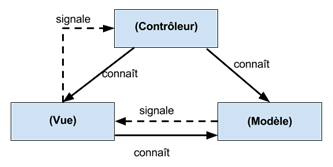
\includegraphics{./img/mvc.png}
            \caption{Patron de conception MVC}
            \label{mvc}
        \end{figure}

        Le modèle (M) représente les données traitées, dans le cas de l’application ce sont principalement les utilisateurs et leur position GPS. Les deux autres composants n’interagissent pas directement avec les données brutes mais ont accès à l’API du modèle symbolisée par le gestionnaire d’utilisateur (UserManager) comme sur la \ref{model}. Le modèle gère donc tous les petits traitements bas niveau sur les données et les sert au reste de l’architecture selon les besoins.

        \begin{figure}[H]
            \centering
            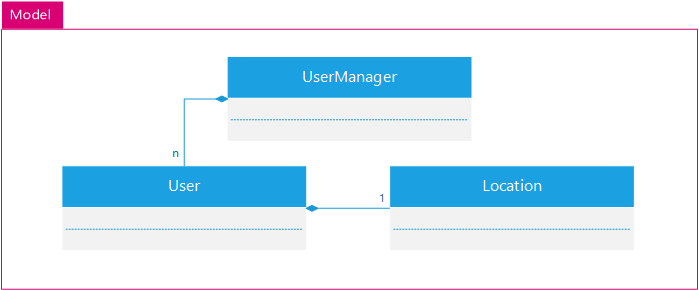
\includegraphics{./img/android-model.png}
            \caption{Diagramme du modèle}
            \label{model}
        \end{figure}

        Le contrôleur (C) s’occupe des interactions avec l’utilisateur, il doit pouvoir transmettre les commandes émanant de l’utilisateur aux autres composants. Dans le cadre de l’application Android, le contrôleur est symbolisé par les activités : ce sont les activités Android qui proposent les interfaces de contrôle utilisateur. Elles permettent de recevoir les évènements utilisateur comme un clic ou encore les messages du système comme l’arrivée d’un SMS ou encore l’actualisation de la position GPS. Les informations reçues peuvent ensuite être utilisées pour effectuer une mise à jour du modèle ou un rafraîchissement de l’affichage. Les différents types d’activités sont visible sur \ref{controller}.

        \begin{figure}[H]
            \centering
            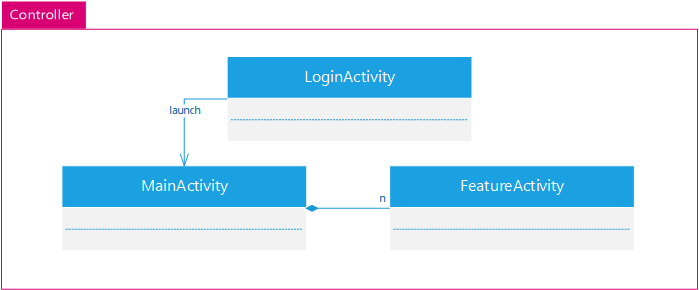
\includegraphics{./img/android-controller.png}
            \caption{Diagramme du contrôleur}
            \label{controller}
        \end{figure}


        La vue (V) est l’ensemble des éléments constituant la façon dont vont être présentées les données. La réalisation concrète dans l’application Android de la vue est faite par les fichiers XML de layout et autres ressources. Dans la vue entre aussi un pan important du concept de l’application : la gestion de l’affichage 3D. En effet, pour la plupart des éléments d’interface, tout peut être géré par des fichiers de métadonnées mais pour générer la carte en trois dimensions d’un lieu il est nécessaire de décrire dans le code la manière d’utiliser les données pour les afficher avec de véritables classes Java. La vue est donc un ensemble complexe constitué de diverses ressources comme on peut le voir sur \ref{view}.

        \begin{figure}[H]
            \centering
            \includegraphics{./img/view-android.png}
            \caption{Diagramme de la vue}
            \label{view}
        \end{figure}

        Le tout s’interconnecte et interagit donc pour faire fonctionner l’ensemble. Mais pour alimenter l’application en données exploitables, des services ont dû être mis en place. Il en existe deux qui servent de sources de données au programme. Le premier est le service GPS, il permet à l’application de récupérer la position du dispositif Android. Dans un premier temps, ce service été basé uniquement sur les données matérielles de l’appareil mais afin d’améliorer la précision, l’utilisation des Google Services a été choisie. Les Google Services utilisent à la fois les données GPS pures mais aussi leur historique ainsi que les données du gyroscope et de l’accéléromètre pour déterminer la position avec une plus grande précision. Ceci s’est avéré indispensable pour une localisation correcte en intérieur.

        Le deuxième service est celui responsable de la communication avec le serveur et qui permet de le requêter. Ainsi ce service permet à la fois d’envoyer sa propre position au serveur mais aussi de récupérer la liste des utilisateurs connectés et leurs informations. Ce service exécute en parallèle du thread principal des requêtes http sur le web service WatchDogZZ. Pour ce faire, il utilise la bibliothèque Volley qui permet d’effectuer simplement des communications sur le réseau.

        Le patron de conception majeur dans ce système applicatif est celui observer-observable : il permet à une des entités d’être prévenue par une autre après inscription qu’un traitement a été effectué. Ceci permet le parallélisme des services et de ne pas bloquer l’interface graphique lors d’un traitement long (communication réseau).

        L’ensemble est sécurisé par le système d’authentification Google. Ce choix a été motivé par la simplicité puisque le client étant sur un système Android, il possède forcément un compte Google associé. Il suffit alors d’effectuer une requête sur les serveurs de Google avec les informations d’authentification de l’appareil pour récupérer un token validant l’identité de l’utilisateur. Ce token est ensuite transmis lors de chaque requête au serveur WatchDogZZ en vue de vérifier l’identité du demandeur (voir la \ref{token}).

        \begin{figure}[H]
            \centering
            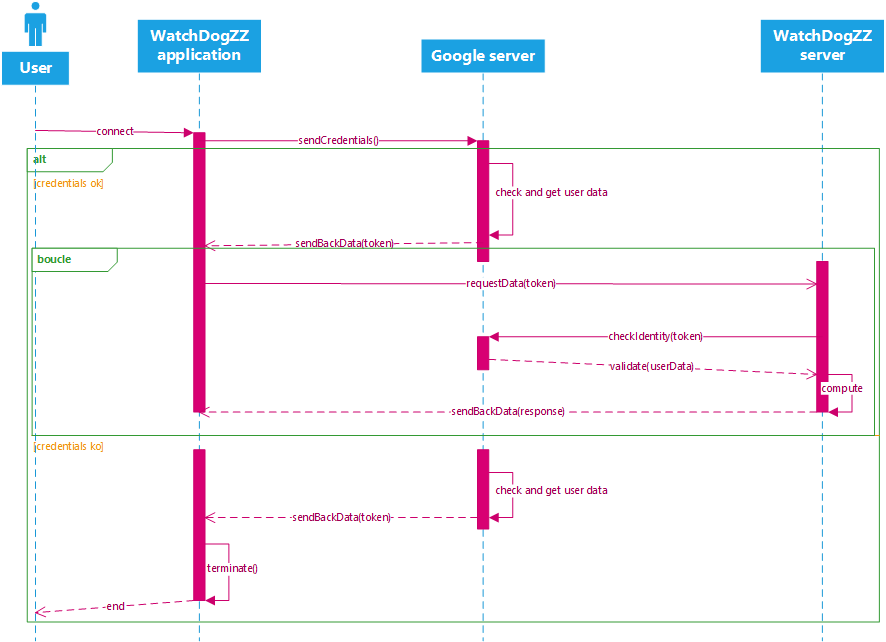
\includegraphics{./img/android-token.png}
            \caption{Utilisation du token Google}
            \label{token}
        \end{figure}

        La carte du maraudeur est une vue qui a été créée spécialement pour l’application. Elle se base sur une SurfaceView reposant sur de l’OpenGL ES 2. L’intérêt était à la fois de pouvoir dessiner en deux mais aussi trois dimensions. Un Renderer spécial a été implémenté ainsi que des managers de ressources 3D. Il est ainsi possible de gérer cette vue comme un observer du UserManager. La vue pourra par la suite afficher les scènes 3D avec les différents éléments à chaque notification. Les différentes classes entrant en jeu sont visibles sur la figure \ref{3d} ainsi que leur rôle dans le MVC.

        \begin{figure}[H]
            \centering
            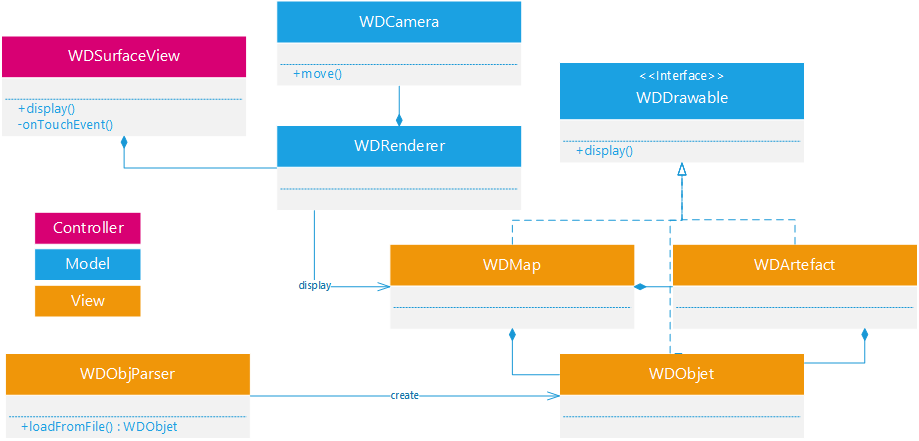
\includegraphics{./img/android-3d.png}
            \caption{Fonctionnement de la 3D Android}
            \label{3d}
        \end{figure}

        La conception de l’application Android est très simple mais fait intervenir de nombreux éléments et services qui touchent énormément d’aspects de la programmation Android. Il existe sur les versions les plus récentes du Framework des fonctionnalités plus intéressantes et performantes toutefois le choix a été fait d’essayer de faire l’application la plus diffusable possible et donc de supporter un maximum d’appareil. Au début du développement, la version choisie était la 9 mais suite à des contraintes inévitables de développement nous avons dû monter à la version 12. Ceci reste correct d’autant plus que cela représente toujours plus de 99% de parts de marché.

        \subsubsection{Web Service}

            Du coté serveur, il faudra gérer plusieurs parties. D'un coté, il faut s'occuper des requêtes utilisateur, et de l'autre, il faut stocker certaines données que l'on renverra aux utilisateurs.
            Pour ce faire, l'architecture est la suivante.

            \begin{figure}[H]
                \centering
                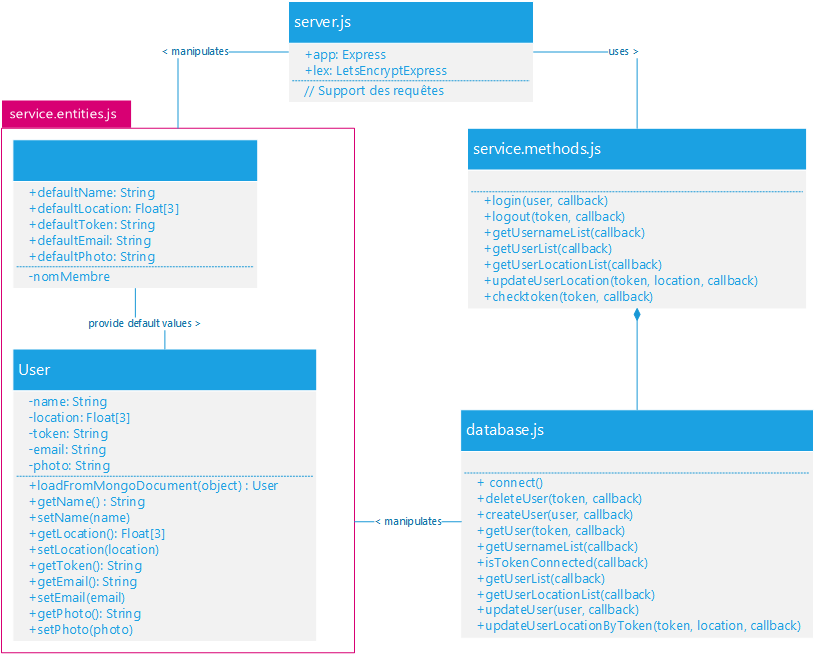
\includegraphics[width=\textwidth]{./img/architecture-service-web.png}
                \caption{Architecture du Service Web}
                \label{asweb}
            \end{figure}

            Comme nous pouvons l'observer dans la figure \ref{asweb}, 


            Le serveur + Mongodb.
            Pattern bridge pour la bdd. Des entités.

    \subsection{Fonctionnalités introduites}

    

    \subsection{Méthodes de développement}

    La méthode adoptée pour la conception de cette solution devait pouvoir convenir à un projet hétérogène et à une équipe de taille faible, un binôme. De façon générale le projet se décomposait en trois sous-projets indépendants : la partie serveur, la partie client et la partie documentation.

    La partie documentation est la seule qui a réellement fait l’objet d’un travail commun avec concertation, échange de points de vue et vérification du travail de l’autre puisqu’elle a consisté en la mise au point des spécifications et en la rédaction de ce rapport. Durant la phase d’analyse et devant l’état des lieux de tout ce qui devait être fait, il a paru équitable et logique de détaché une personne sur le projet Android et une autre sur le projet serveur. Ainsi la répartition des tâches et l’expertise sur les différents projets étaient très contrôlé.

    Une fois que les besoins de l’application ont été analysés et que les spécifications ont été posées, nous avons transformé ses documents en un kanban regroupant les user stories principales. Ces user stories forment l’ensemble minimal des tâches à effectuer pour avoir une application fonctionnelle répondant aux demandes fondamentales du cahier des charges. Dès lors que cette sélection a été faite, le développement des projets primitifs du client et du serveur a commencé. Des échanges réguliers sur les outils de travail d’équipe de GitHub, que nous détaillons plus loin, ont permis de suivre l’évolution du développement linéaire de chaque projet et de rendre compte du travail effectué. L’objectif de cette période était donc de livrer une version fonctionnelle de l’application pour la mi-janvier.

    Au terme de cette première période nous avons pu livrer une application répondant aux critères minimaux et permettant de suivre des personnes dans l’ISIMA. En partant de cette base fonctionnelle nous avons commencé le développement de fonctionnalités plus poussées avec une méthode un peu différente : une méthode plus agile.

    Nous avons listé tous les bugs connus, les améliorations et les fonctionnalités que nous souhaitions ajouter. Ensuite nous avons commencé à fonctionner en itérations agiles d’une durée de deux semaines. En début d’itérations nous sélectionnions un ensemble d’items qui étaient des « issues » sur GitHub et nous en faisions une milestone. Nous travaillions ensuite sur ces issues et en fin de cycle nous faisions le point sur l’itération terminée et nous rajoutions des issues en fonction de la situation. Le développement agile a permis de rajouter des fonctionnalités avancées sur deux ou trois itérations.

    L’ensemble de ces éléments fait que nous avons pu développer étape par étape une application qui semblait très complexe à mettre en place. Sans cette méthode nous aurions peut-être été perdu devant tout le travail mais dans les faits, malgré quelques difficultés nous avions toujours une version fonctionnelle qui répondait aux critères minimaux du cahier des charges.